\section{Numerical implementation of the equilibrium solver}\label{app:solver_details}

The equilibrium solver works in EUR billions and includes the full accounting estate. Let $\mathbf{B}=(x_{ij})_{i,j\in\mathcal B}$ be the bank claim matrix, $\mathbf{D}=(D_i)$ the clearing-debt vector, and $\mathbf{a}(s)=(a_i(s))$ the net nonbank-resource vector from Section~\ref{sec:model_banks}. All $a_i(s)$ are strictly positive in the calibration. The cutoff $T_i$ is defined in the same section. Appendix~\ref{app:calibration-details} explains how these resources and debts are reconciled to the data. The NBFI balance-sheet check establishes par repayment in this calibration; an independent eight-node enumeration verifies selected results with endogenous NBFIs.

\paragraph{Uniqueness without default costs}
At $\lambda_i^B=1$, write total bank payments as $p_i=D_iR_i$ and define the internal liability shares $\Pi_{ij}=B_{ji}/D_i$: rows are debtors and columns creditors. Collect these shares in $\boldsymbol{\Pi}=(\Pi_{ij})$ and payments in $\mathbf{p}=(p_i)$, with transpose denoted by $\top$. The bank-only clearing map is
\[
 \Psi_s(\mathbf{p})=\min\{\mathbf{D},\mathbf{a}(s)+\boldsymbol{\Pi}^\top \mathbf{p}\},
\]
The minimum is componentwise. The debt share owed within the bank block is $\ell_i=\sum_j\Pi_{ij}$. If $\ell_i<1$ for every bank, some payment from every bank goes to outside creditors. For any two payment vectors $\mathbf{p},\mathbf{p}'$, the $\ell_1$ norm satisfies
\[
 \|\Psi_s(\mathbf{p})-\Psi_s(\mathbf{p}')\|_1
 \leq\|\boldsymbol{\Pi}^\top(\mathbf{p}-\mathbf{p}')\|_1
 \leq\left(\max_i\ell_i\right)\|\mathbf{p}-\mathbf{p}'\|_1.
\]
Thus the map is a contraction and the clearing vector is unique for every nonnegative $\mathbf{a}(s)$. This is a strong sufficient condition for the open bank block, not a necessary condition. Internal debt shares are 16.1\%, 17.0\%, 10.6\% and 7.4\% for Germany, France, Italy and Spain, giving a contraction factor below .18. Clearing debt here excludes fixed outside settlements but retains the nonbank creditors sharing ordinary bank repayment. Gross domestic bank claims remain internal to $\boldsymbol{\Pi}$. With default costs, the map remains contractive within each fixed default regime, but jumps between regimes can prevent global contraction.

\paragraph{Regularity in the original clearing model}
Conditional on a sovereign state and fixed nonbank receipts, the no-cost model has fixed nominal debts, proportional sharing, debt priority over equity and no value destruction at default. Monotonicity gives existence; uniqueness requires an additional condition. In the closed-network formulation of \citet{EisenbergNoe2001}, regularity requires every node's risk orbit---the node and its direct or indirect creditors---to contain positive external resources. Strictly positive external resources at every node are a simple sufficient condition.\footnote{See their Definitions 2--5 and Theorem 2. Paths follow liabilities from debtor to creditor, the reverse of the creditor-to-debtor arrows in our exposure figure. These are sufficient conditions, not necessary conditions for uniqueness.} This excludes closed payment circuits with no external resources to anchor settlement. For example, if two banks owe one unit to each other, have no outside assets and owe nothing outside the pair, any common payment between zero and one clears their obligations. A cycle of obligations can therefore admit indeterminate payments when it has no external anchor. The outside-creditor condition above provides a direct contraction argument for our open bank block; its fixed net external receipts are also positive in all sixteen states.

\paragraph{Default-set enumeration}

For each of sixteen sovereign states, enumerate the sixteen bank default sets $J\subseteq\mathcal B$, with complement $J^c=\mathcal B\setminus J$. The operator $\operatorname{diag}$ forms a diagonal matrix. Subscripts on vectors and matrices select the indicated banks; $\mathbf1$ is a vector of ones and $\mathbf{I}$ an identity matrix of matching dimension. With $\boldsymbol{\Gamma}_J=\operatorname{diag}(\lambda_i^B/D_i)_{i\in J}$, ordinary repayment solves
\[
 [\mathbf{I}-\boldsymbol{\Gamma}_J\mathbf{B}_{JJ}]\mathbf{R}_J
   =\boldsymbol{\Gamma}_J[\mathbf{a}_J(s)+\mathbf{B}_{J,J^c}\mathbf1].
\]
Retain a solution only if $0\leq R_i<1$ and $A_i<T_i$ for $i\in J$, while $R_i=1$ and $A_i\geq T_i$ otherwise. The default check is prudential, not a check that accounting equity is exhausted. Equality belongs to full repayment. Enumeration requires nonsingular candidate systems; the implementation reports an error if this condition fails.

\paragraph{Policy regions}
Let $\eta_j$ denote the backstop coverage assigned to debtor $j$: common coverage $\eta$ for eligible banks and zero for excluded banks. Effective creditor repayment is $\max\{R_j,\bar R_j(s)\}$ under a floor and $\min\{1,\mu_jR_j\}$ on the default branch under a recovery backstop, where $\mu_j=1+\eta_j(1-\lambda_j^B)/\lambda_j^B$. In each binding-floor or binding-cap region, write creditor repayment $d_j+\gamma_jR_j$, where $d_j$ and $\gamma_j$ are that region's intercept and slope. Collect the intercepts in $\mathbf{d}=(d_j)$ and let $\boldsymbol{\gamma}_J=(\gamma_j)_{j\in J}$. The candidate system is
\begin{equation}
 [\mathbf{I}-\boldsymbol{\Gamma}_J\mathbf{B}_{JJ}\operatorname{diag}(\boldsymbol{\gamma}_J)]\mathbf{R}_J
    =\boldsymbol{\Gamma}_J[\mathbf{a}_J(s)+\mathbf{B}_{J,\mathcal B}\mathbf{d}],
 \label{eq:interbank_backstop_linear_system}
\end{equation}
where $\mathbf{a}(s)$ is the fixed external receipt vector defined above. Nondefaulting debtor entries have slope zero and intercept one. Enumerate every region and check its floor/cap inequalities and the original repayment map. Identical boundary roots are counted once. Zero floors and zero backstop coverage reproduce the baseline.

The preferred equilibrium maximizes summed ordinary repayments and is the greatest fixed point of the monotone map. Proposition~\ref{prop:greatest-floor} ensures that the floor leaves exactly that equilibrium and pays zero; enumeration verifies this in every state. Proposition~\ref{prop:critical-floor-budget} characterizes the critical capacity of the proportional capped floor. The online appendix gives its proof and the finite default-regime calculation, including the endpoint test. Expected results assign weight $1-\rho$ to the highest-sum repayment root and share $\rho$ equally among other roots, using $\rho=.20$ for the reference; unique states receive weight one. Sovereign-state probabilities are products of the calibrated default/survival probabilities.

\section{Data, accounting and calibration}\label{app:database_construction}\label{app:calibration-details}

\subsection{Source coverage and balance-sheet reconciliation}

The Online Appendix explains the public source hierarchy, missing bilateral allocations and the treatment of related offices. The 24-account reporting matrix preserves the rest of the world and unidentified holders and issuers separately. The model groups them into Other counterparties without netting claims; the Eurosystem remains separate. Figure~\ref{fig:full-exposure-network} shows the resulting 22-node network, complementing the bank-focused view in Section~\ref{sec:calibration}. Figure~\ref{fig:active_source_matrix} records source coverage.

\begin{figure}[htbp]
\centering
\floatcaption{Residence-based exposure network, end-2024}{Bk = banks; Gvt = government; NBFI = nonbank financial institutions; Firm = firms; HH = households. Arrows run from creditor to debtor and retain the five largest outgoing claims per node; calculations use the full network. Thickness increases with the claim size in EUR billions. Colours identify countries or aggregate blocks. Gross domestic bank claims are retained in clearing but omitted from this drawing; Figure~\ref{fig:calibrated-exposure-network} displays them as loops.}
\label{fig:full-exposure-network}
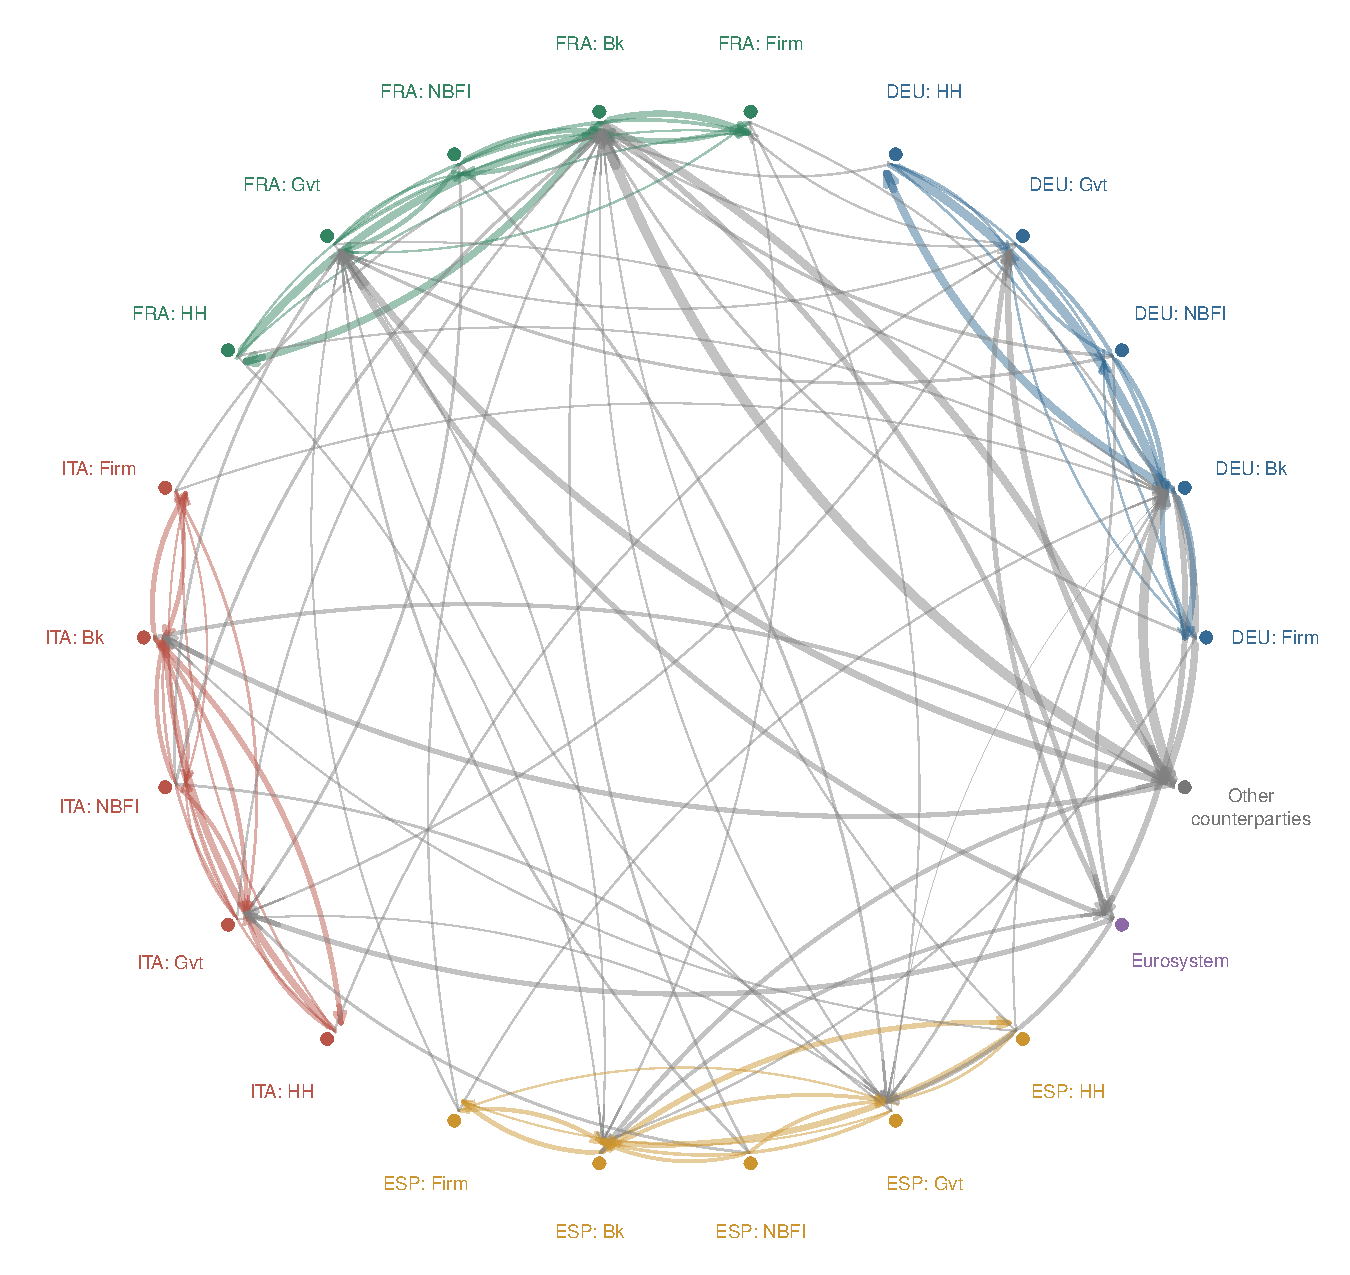
\includegraphics[width=\textwidth]{Figures/figure_network_2024-10-01.pdf}
\end{figure}

\begin{figure}[htbp]
\centering
\floatcaption{Sources represented in the end-2024 residence matrix}{Rows are creditors and columns are debtors. White cells have no positive claim. Cells combining different source layers are marked ``Multiple sources''. Detailed source keys, amounts and reconciliation rules remain in the exposure register.}
\label{fig:active_source_matrix}

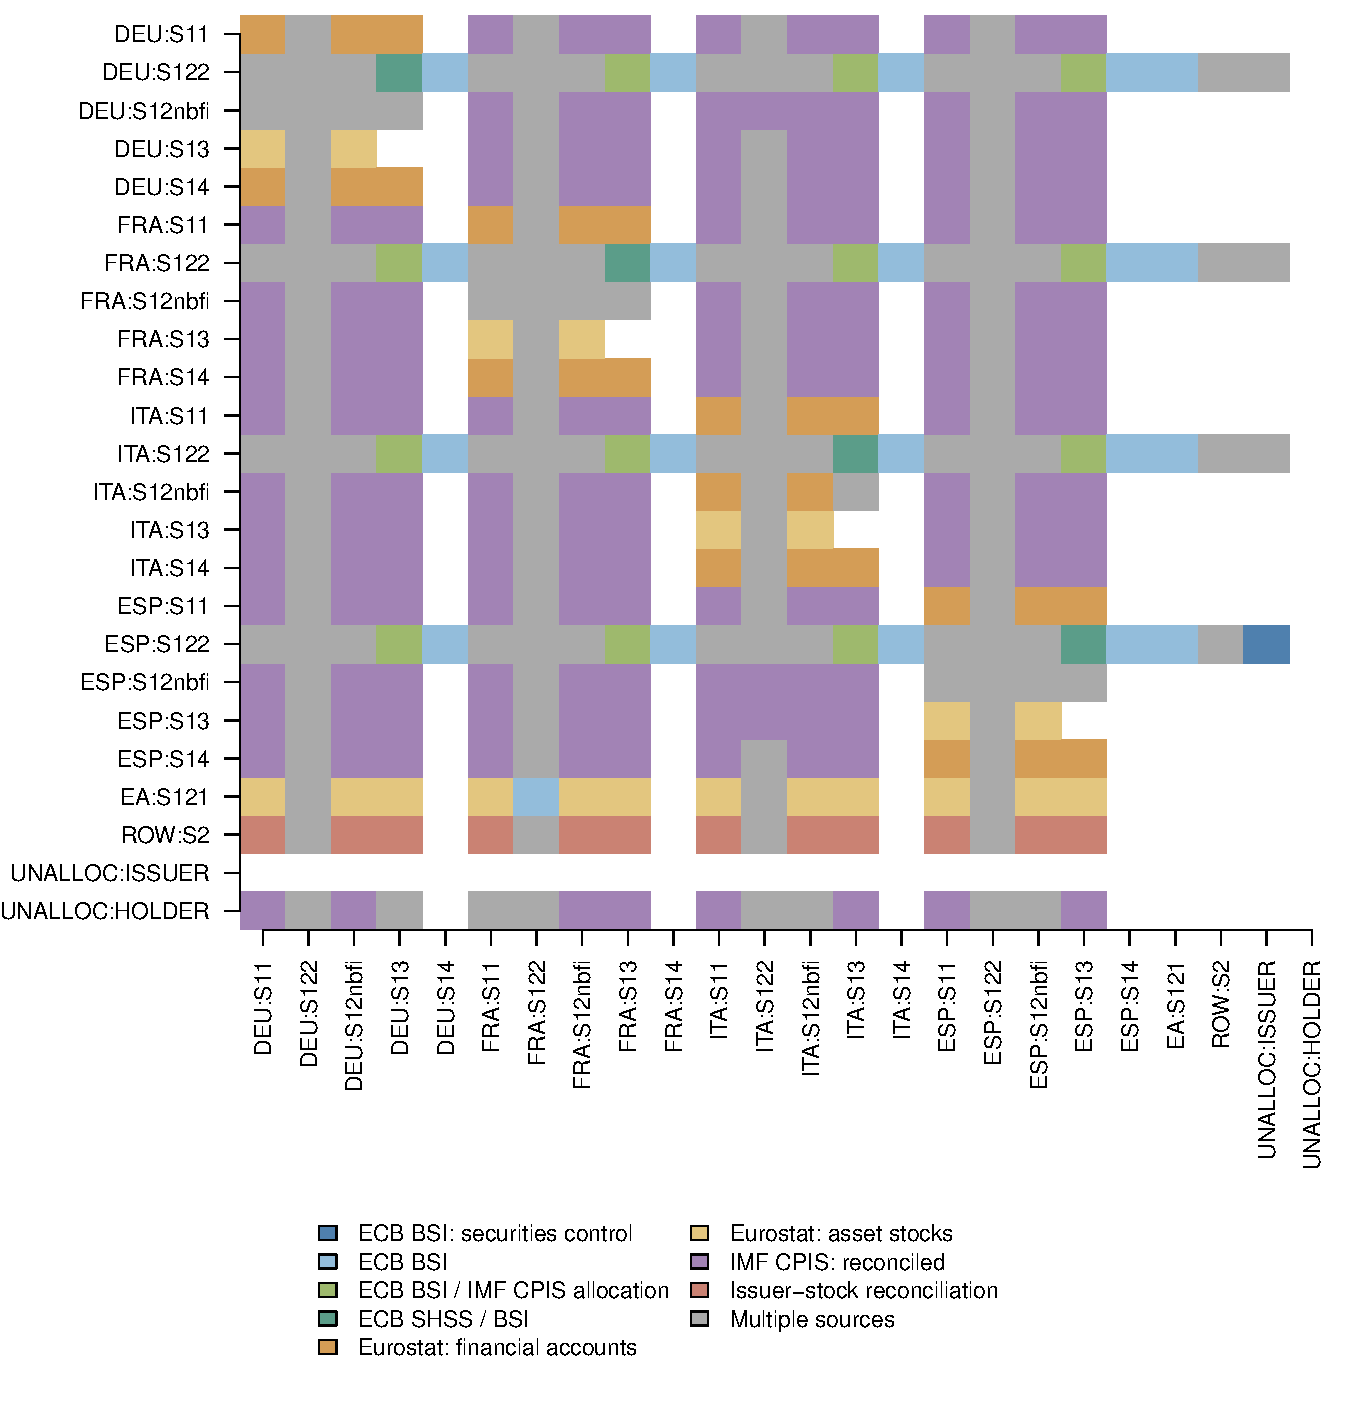
\includegraphics[width=\textwidth]{Figures/active_source_matrix_2024-10-01.pdf}

\end{figure}

The matrix covers selected loans, deposits and debt securities. Other bank assets include government loans, equity holdings, nonfinancial assets and items whose bilateral counterparties are not reconstructed. Coverage and valuation adjustments reconcile these positions to reported balance sheets. Net positions remaining after identified related-office claims are removed are also retained in the reconciliation. These items supply reference repayment resources; they are not independently measured productive wealth.

Write $B_{ij}=x_{ij}$ for banks $i,j$, and $N_{ig}=x_{i,G_g}$ for bank $i$'s holdings of country $g$'s sovereign bonds. Let $D_i^*$ be adjusted statistical liabilities, and let $O_i$ collect net group funding, central-bank funding and remaining or unclassified outside funding settled separately from the common pool. Set
\[
 D_i=D_i^*-O_i,\qquad
 b_i=D_i+E_i-\sum_jB_{ij}-\sum_gN_{ig},
\]
The reference resources therefore satisfy
\[
 b_i+\sum_jB_{ij}+\sum_gN_{ig}=D_i+E_i.
\]
The common pool contains deposits and issued securities. Fixed outside settlements reduce both debt and resources. Provisions against assets are deducted from statistical capital and gross assets together, leaving accounting equity $E_i$. The reference amount $b_i$ includes performing nonbank receipts, outside assets, government loans and coverage or valuation adjustments, net of fixed settlements.

This convention preserves equity but does not assert that the public data identify a single legal recovery class. Remaining liabilities include derivatives and settlement positions, with incomplete public information on close-out rank. The Online Appendix reports the adjustments and statistical-liability benchmarks separately.

\subsection{Prudential headroom and full accounting equity}

For each significant institution, we compute the smaller loss capacity above its published overall risk-weighted capital stack and its leverage requirement. Writing CET1 for Common Equity Tier 1 capital, the country median headroom/CET1 ratio is transferred to resident accounting equity using the same country's public supervisory CET1/equity bridge. Table~\ref{tab:ocr-headroom} reports the resulting headroom and the alternative capacity above a 4.5\% CET1 floor. Consolidated significant institutions and resident offices have different perimeters; these are labelled country proxies, not measured resident regulatory capital.

\begin{table}[htbp]
\centering
\floatcaption{Accounting equity and prudential headroom (EUR billions)}{Equity and clearing debt follow the resident bank balance-sheet reconciliation. OCR headroom uses end-2024 public ECB Pillar 3 and supervisory statistics. ISA headroom is the alternative proxy above a 4.5\% CET1 floor. Neither headroom is substituted for accounting equity in the repayment estate.}
\label{tab:ocr-headroom}
\small

\begin{tabular*}{\textwidth}{@{\extracolsep{\fill}}lrrrr@{}}
\toprule
Country & Accounting equity & Clearing debt & OCR headroom & ISA headroom \\
\midrule
DEU & 686.4 & 7453.6 & 196.8 & 395.5 \\
FRA & 657.0 & 7987.6 & 208.3 & 365.1 \\
ITA & 331.2 & 2697.1 & 90.6 & 168.6 \\
ESP & 245.7 & 2415.9 & 61.5 & 124.5 \\
\bottomrule
\end{tabular*}


\end{table}

Losses exceeding headroom satisfy the first condition for a costly credit event under the disorderly-crisis scenario. An OCR breach can restrict distributions without causing legal default. Market stigma, funding pressure and overlapping constraints can nevertheless impede buffer use \citep{ECBBuffer2023,ECBESRB2026}. The scenario assumes no timely recapitalization or relaxation sufficient to prevent distress. All remaining accounting equity stays in the repayment estate; headroom is never substituted for equity. Partial repayment additionally requires a shortfall after the distress cost.

At the normalized contractual return one, the distress cutoff is $T_i=\min\{D_i+E_i-H_i,D_i/\lambda_i^B\}$. The first term imposes headroom exhaustion; the second ensures that creditors receive less than par on the default branch. Equality gives full repayment. With $H_i=E_i$, the trigger is accounting insolvency; with $\lambda_i^B=1$, the rule becomes ordinary capped pro-rata clearing for any $H_i\leq E_i$.

The baseline $\lambda_i^B=.90$ follows the 10\% remaining-asset default cost in the systemic bank-stress model of \citet{Aikman2009}. It represents realization and franchise disruption in addition to initial credit losses. It is a modelling benchmark, not an estimate of contemporary European administrative resolution costs.

\subsection{Sovereign and private-credit losses}

Safe and contractual bank gross returns equal one. Let $\pi_g^G$ be country $g$'s calibrated annual sovereign-default probability. With 50\% recovery of the contractual payment, sovereign repayments are
\[
 R_g^G(s)=\frac{1-.5\delta_g^G(s)}{1-.5\pi_g^G}.
\]
Mean five-year CDS quotes over December 2007--November 2025 are 14.8, 27.9, 102.5 and 83.9 basis points for Germany, France, Italy and Spain. Let $s_g$ denote these spreads in decimal form. We use them as annual contractual yield-spread proxies, setting $\overline r_g^G=1+s_g$. The expected-payoff normalization $(1-.5\pi_g^G)\overline r_g^G=1$ then gives $\pi_g^G=s_g/[.5(1+s_g)]$, approximately 0.30\%, 0.56\%, 2.03\% and 1.66\%. This is a one-period pricing convention; CDS premium schedules and maturity are not priced separately. These are market-price-based inputs, not historical default frequencies. Marginal risk inputs affect the sovereign payoff normalization; the state comparisons condition on that payoff grid.

The private-credit shock follows the borrower's country. Let $i$ index the creditor's national bank block and $g$ the borrower's country, each among Germany, France, Italy and Spain. The $4\times4$ matrices $\mathbf{F}$ and $\mathbf{Q}$ record bank loans to nonfinancial firms and households, respectively: $F_{ig}$ is the amount lent by banks in country $i$ to firms in country $g$, and $Q_{ig}$ is the corresponding amount lent to households. These loan stocks are extracted from the exposure register; they exclude securities included in the broader sector exposures.

If sovereign $g$ defaults, the scenario imposes an additional loss on those private loans of
\[
 \mathcal L_{ig}=.018F_{ig}+.017Q_{ig}.
\]
For example, a French sovereign default generates private-credit losses for German banks on their loans to French firms and households, even if Germany's sovereign does not default. Summing across borrower countries gives bank $i$'s additional private-credit loss, $\sum_g\mathcal L_{ig}\delta_g^G(s)$, where $\delta_g^G(s)$ equals one if sovereign $g$ defaults in state $s$ and zero otherwise. Its resources before interbank receipts are therefore
\[
 a_i(s)=b_i+\sum_gN_{ig}R_g^G(s)-\sum_g\mathcal L_{ig}\delta_g^G(s).
\]
The sovereign-bond receipts in the second term and the private-loan losses in the third term are distinct channels. The private loss rates, 1.8\% for firm loans and 1.7\% for household loans, are pooled adverse-minus-baseline impairment proxies from the ECB's 2025 bank stress test, Chart 3.8 \citep{ECBStress2025}. Applying them in borrower-country sovereign-default states is a scenario assumption, not an estimated causal relationship. They capitalize a three-year episode once at settlement. Government loans, private securities and outside-sample private loans receive no additional impairment. Opening equity is already net of provisions, so the provision stock is not deducted again. Credit supply and private borrowing remain fixed.

\subsection{NBFI repayment and gross domestic bank claims}

NBFIs have pooled public financial-account buffers and no additional default cost. Financial assets less non-equity liabilities exceed the complete selected bank, NBFI and sovereign claims by approximately EUR~3,500 billion in Germany, 1,329 billion in France, 228 billion in Italy and 377 billion in Spain. With national pooling and other net resources fixed, even zero receipts on these claims leave ordinary debt covered. This establishes par repayment in every equilibrium. An independent eight-node enumeration verifies selected results. Halving NBFI buffer availability also leaves all reported bank equilibrium vectors unchanged.

Identified related-office loans are removed with matched balance-sheet adjustments. The remaining domestic bank claims are retained in $B_{ii}$ as gross obligations among distinct institutions sharing the national repayment rate. The Online Appendix gives a symmetric disaggregation into institutions without own claims that reproduces the block map exactly. It does not rule out asymmetric institutional outcomes. Netting these claims and equal liabilities changes the clearing representation and the estate exposed to costs; this diagnostic removes baseline multiplicity.

\subsection{Weights and comparison with ISA}

Sovereign defaults are independent for the limited set of averages across states reported in the paper; Appendix~\ref{app:ocr_robustness}, Table~\ref{tab:sovereign-dependence}, reports a dependence sensitivity for recovery-backstop averages. In a state with several banking equilibria, the greatest repayment vector receives weight $1-\rho$ and the remaining roots share $\rho$ equally, with $\rho=.20$. A unique root receives weight one. The debt-weighted expected ordinary bank repayment shortfall is approximately 3.0 basis points. State-specific clearing and the maximum capacity over all states do not use these selection weights or the independence convention.

The ECB's Interconnected System-wide stress test Analytics (ISA) application combines granular supervisory and commercial data with liquidity and asset-price feedback \citep{GrassiEtAl2025}. Our public resident-sector network isolates repayment feedback and guarantee capacity. ISA's 4.5\% CET1 default threshold motivates our alternative headroom specification in Appendix~\ref{app:ocr_robustness}, Table~\ref{tab:ocr-robustness} (the row labelled ``ISA headroom''); the baseline uses public OCR/leverage headroom as a conditional distress trigger. The private-credit proxies come from the separate bank stress-test report, not ISA's contagion results. The Online Appendix compares their coverage and thresholds.


\section{An optional household completion}\label{app:household-completion}\label{app:calibration_implementation}

The clearing analysis takes exposures and reference repayment resources as given. This appendix describes a household-saving model that can interpret those positions and their consumption incidence. It is not used to determine exposures, calibrate bank resources or solve any of the reported policy experiments.

\subsection{Complete accounts and household saving}\label{sec:model_households}

Consider complete date-1 accounts. Node $i$ has initial resources $e_i$, absorption $C_i$, lending $X_i=\sum_jx_{ij}$ and borrowing $D_i=\sum_jx_{ji}$. Set $\alpha_{ij}=x_{ij}/X_i$ when $X_i>0$, and use any nonnegative portfolio-share row summing to one when $X_i=0$. Bold symbols denote vectors, and $\boldsymbol\alpha=(\alpha_{ij})$ is the portfolio-share matrix. The accounts satisfy
\[
 e_i+D_i=C_i+X_i,\qquad
 \mathbf D=\boldsymbol\alpha^\top\mathbf X,
 \qquad \mathbf e=\mathbf C+\mathbf X-\mathbf D.
\]
Set $C_{H_c}=c_{1,c}$ and $C_i=0$ for other nodes. These identities concern complete accounts; the selected empirical network instead uses the bank reconciliation to supply omitted resources, clearing debt and accounting equity. Initial resources $e_i$ are distinct from bank accounting equity.

Let $Y_{2,c}(s)$ be nonportfolio resources, $P_{H_c}(s)$ the household debt payment, $\beta>0$ the discount factor, and $u_c^0,u_c^1,u_c^2$ utility coefficients, with $u_c^2>0$. Let $r$ and $r^R$ denote the reference private and safe gross returns, both normalized to one in the quantitative exercise. These resources and debt payments are given. The reference debt payment is $rD_{H_c}$; scenario payments may reflect the specified impairment of bank-held household loans. On household-held claims, $R_j$ is the realized government or bank repayment when the debtor is a sovereign or bank, $r$ for the other domestic sectors under the baseline par-repayment result, and $r^R$ for the Eurosystem and Other counterparties. Instrument-specific scenario payoffs can be incorporated without changing the saving argument.

Household $H_c$ takes borrowing, portfolio shares and the distribution of claim repayments as given. It chooses $c_{1,c}\geq0$ and $X_{H_c}\geq0$ to maximize
\[
 u_c(c_{1,c})+\beta\mathbb E[c_{2,c}],\qquad
 u_c(c)=u_c^0+u_c^1c-\frac{u_c^2}{2}c^2,
 \quad u_c^2>0,\quad\beta>0,
\]
subject to
\[
 e_{H_c}+D_{H_c}=c_{1,c}+X_{H_c},\qquad
 c_{2,c}(s)=Y_{2,c}(s)+X_{H_c}\sum_j\alpha_{H_c,j}R_j(s)-P_{H_c}(s).
\]

The objective is strictly concave in $c_{1,c}$, with second derivative $-u_c^2<0$. At an interior solution, $u_c^1-u_c^2c_{1,c}=\beta\mathbb E[\sum_j\alpha_{H_c,j}R_j]$, giving
\[
 X_{H_c}=e_{H_c}+D_{H_c}-\frac{u_c^1}{u_c^2}
       +\frac{\beta}{u_c^2}\mathbb E\!\left[\sum_j\alpha_{H_c,j}R_j\right].
\]
This condition is not imposed in calibration or clearing: exposures are observed or reconstructed inputs. The completion does not model firms' portfolio choices or credit-supply responses.

\subsection{Consumption and utility differences}

Fix a sovereign state and compare two banking equilibria with identical portfolios, debt payments and nonportfolio resources. Their date-2 consumption difference equals their receipt difference. With NBFIs repaying in full, only bank payments vary, yielding the expression in Section~\ref{subsec:household-macro-implications}.

With date-1 consumption fixed, full pass-through of receipts to date-2 consumption and no other transfers or financing costs, the conditional utility gain from selecting the preferred equilibrium is $\beta\Delta c_{2,c}^e(s)$. Deposit protection and its financing can change that incidence. These assumptions do not turn gross receipt differences into estimates of realized consumption or welfare gains; neither consumption levels nor preference parameters enter their calculation.


\section{Robustness of the crisis specification}\label{app:ocr_robustness}

Table~\ref{tab:ocr-robustness} varies public headroom definitions and selected crisis assumptions while preserving the residence matrix and full bank accounting equity. All cases use $\lambda=.90$ except the minimum-requirement row. In 75 joint local combinations, OCR headroom varies from 90\% to 110\% of its reference value, $\lambda$ from .89 to .91, and both private-loss rates by $\pm.1$ percentage point. Multiplicity persists in 3--10 states throughout; defaults under full interbank repayment occur in twelve states and the no-sovereign-default state stays unique. These are scenario sensitivities, not confidence intervals.

\begin{table}[htbp]
\centering
\floatcaption{Public-threshold and crisis sensitivities}{Default states count sovereign states with at least one bank default under full interbank repayment; bank--state events count individual bank-country/state pairs with such defaults. This diagnostic applies sovereign and private-credit losses while assuming full payment of every interbank claim. All counts concern sixteen sovereign states. Lower/upper quartiles describe cross-bank headroom ratios; they are not estimated national confidence bounds. NBFI availability of 50\% leaves all bank equilibrium vectors unchanged.}
\label{tab:ocr-robustness}
\small

\begin{tabular*}{\textwidth}{@{\extracolsep{\fill}}lrrr@{}}
\toprule
Specification & Default states & Bank--state events & Multiple states \\
\midrule
ISA headroom, $\lambda=.90$ & 12 & 16 & 0 \\
Half ISA headroom, full equity & 12 & 22 & 3 \\
Public median OCR (baseline) & 12 & 16 & 8 \\
Lower-quartile OCR & 14 & 24 & 8 \\
Upper-quartile OCR & 12 & 16 & 6 \\
Minimum requirements, $\lambda=.875$ & 12 & 16 & 8 \\
Sovereign recovery 55\% & 12 & 16 & 8 \\
Sovereign recovery 45\% & 12 & 16 & 7 \\
NBFI availability 50\% & 12 & 16 & 8 \\
\bottomrule
\end{tabular*}


\end{table}

Admitting 25\%, 50\%, 75\% and 100\% of the capacity between OCR and minimum requirements leaves 8, 6, 4 and 2 multiple states, respectively. With a 5\% default cost, multiplicity disappears. Netting domestic bank claims and equal liabilities also removes multiplicity, showing the role of gross domestic exposures. The online appendix provides their symmetric-institution interpretation.

\paragraph{Average losses and payments under the recovery backstop}
Section~\ref{sec:interbank-recovery-backstop} reports state-by-state equilibrium effects and maximum payments. Figure~\ref{fig:backstop-weighted-averages} additionally summarizes average outcomes. In each sovereign state, the preferred policy equilibrium receives weight $1-\rho$ and the others share $\rho$ equally; a unique equilibrium receives weight one. We consider $\rho\in\{.1,.2,.3\}$. Crisis-conditional averages then weight sovereign states using the independent marginal risk inputs from Section~\ref{subsec:calibration_choices}. Interbank credit loss is the claim-weighted shortfall $\sum_jL_j^{BB}[1-\widehat R_j^e(s;\eta)]/\sum_jL_j^{BB}$. A state-expected payment averages over equilibria within a given sovereign state; its maximum across states can differ from the maximum across individual equilibria reported in the main text.

At half coverage and $\rho=.20$, payments conditional on a sovereign crisis are 0.05\% of aggregate bank debt, and conditional interbank credit losses fall from 44.2 basis points without intervention to 3.1 basis points. Since half coverage gives a unique equilibrium in every sovereign state, its policy outcomes do not depend on $\rho$; the comparison without intervention does. Dependence between sovereign defaults affects these crisis-conditional averages, as examined below.

\begin{figure}[htbp]
\centering
\floatcaption{Recovery-backstop averages under alternative equilibrium-selection weights}{Coverage is evaluated in five-percentage-point steps and $\rho\in\{.1,.2,.3\}$. Panel (a) counts states with multiplicity. Panels (b) and (c) report interbank credit losses and payments conditional on a sovereign crisis under independent defaults. Panel (d) gives the largest within-state expected payment. Payments are percentages of aggregate bank debt; interbank losses are basis points of interbank claims.}
\label{fig:backstop-weighted-averages}

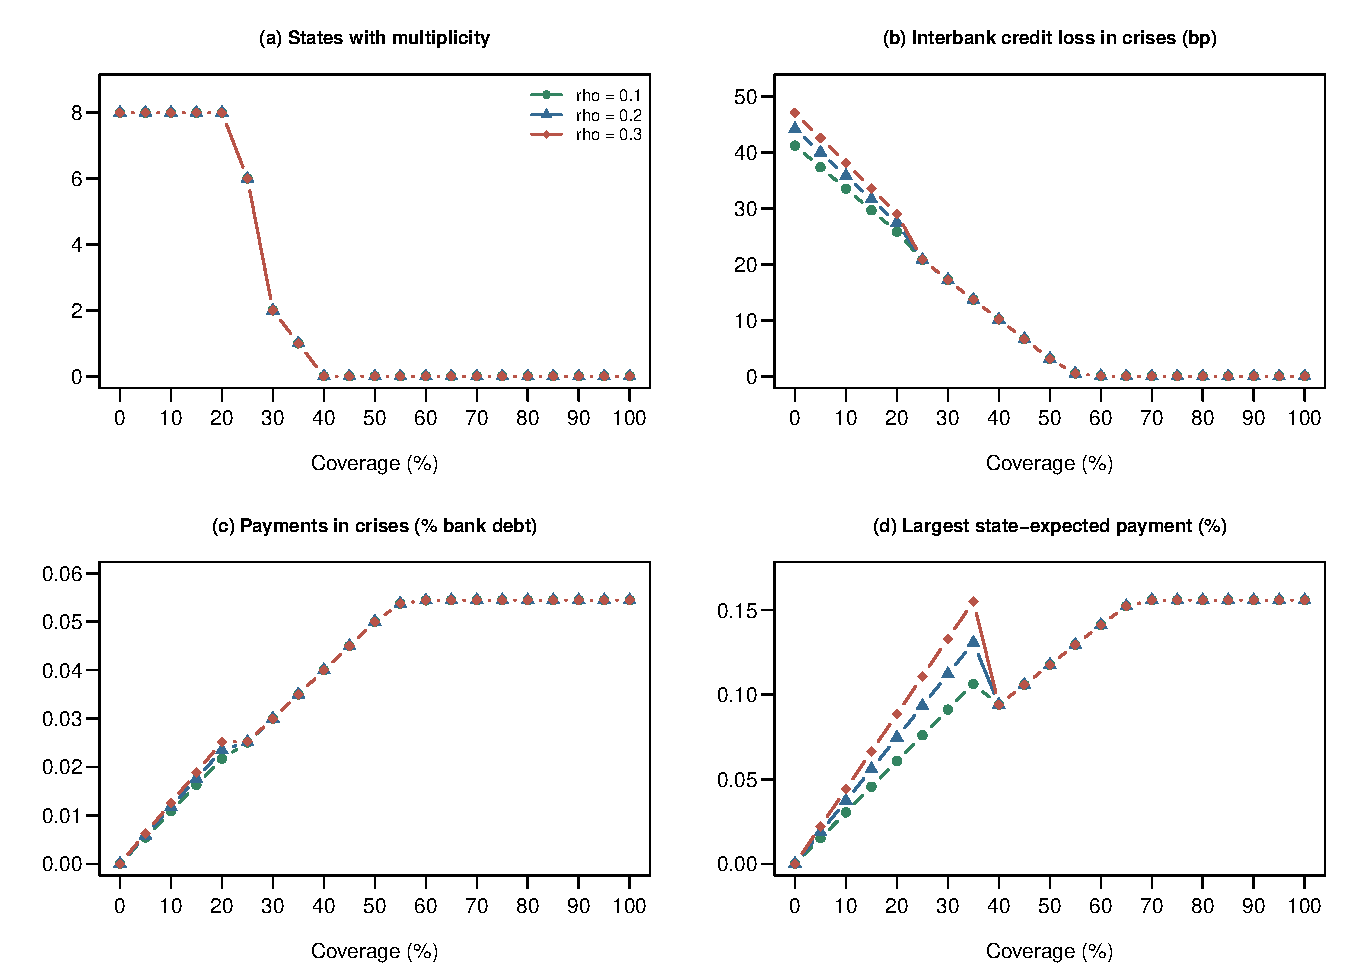
\includegraphics[width=\linewidth]{Figures/interbank_recovery_backstop_averages.pdf}

\end{figure}

\paragraph{Dependence between sovereign defaults}
Independence affects averages across sovereign states, not the equilibrium solutions conditional on a state. Table~\ref{tab:sovereign-dependence} reweights the saved equilibria while keeping each country's marginal default probability, sovereign payments and within-state equilibrium weights ($\rho=.20$) fixed. We mix independence with a shared-shock distribution: for a single uniform random variable $U$, country $g$ defaults when $U<\pi_g^G$. A mixture weight of one is the fully shared-shock case.\footnote{For the 50--50 mixture, imagine tossing a single fair coin for all four countries, before conditioning on a sovereign crisis. On heads, their defaults are independent, with the calibrated probabilities: approximately 0.30\% for Germany, 0.56\% for France, 2.03\% for Italy and 1.66\% for Spain. On tails, draw a single $U$ uniformly between zero and one and compare it with each country's default probability. For example, $U=0.4\%$ implies default in France, Italy and Spain, while $U=1\%$ implies default only in Italy and Spain. Defaults are thus nested under the shared shock: whenever a lower-risk sovereign defaults, all higher-risk sovereigns default too. Each sovereign configuration receives half its probability under independence plus half its probability under the shared shock. Each country's individual default probability is unchanged because it is the same under both mechanisms. The 50\% is the probability of selecting the shared-shock mechanism, rather than a default correlation of 50\%.} This is a dependence stress, not an estimate of sovereign correlations.

\begin{table}[htbp]
\centering
\floatcaption{Sovereign-dependence sensitivity of recovery-backstop averages}{B--B losses and payments are conditional on at least one sovereign default. Losses are basis points of interbank claims; payments are percentages of aggregate clearing debt. The shared-shock weight changes the joint distribution while preserving marginal default probabilities. All state-specific equilibria and all-state commitment capacities remain unchanged.}
\label{tab:sovereign-dependence}
\small

\begin{tabular*}{\textwidth}{@{\extracolsep{\fill}}lrrrr@{}}
\toprule
Dependence & \shortstack{Crisis probability\\(\%)} & \shortstack{B--B loss\\$\eta=0$ (bp)} & \shortstack{B--B loss\\$\eta=.50$ (bp)} & \shortstack{Payment\\$\eta=.50$ (\% debt)} \\
\midrule
Independent & 4.48 & 44.2 & 3.1 & 0.05 \\
50\% shared-shock mixture & 3.26 & 65.5 & 8.1 & 0.07 \\
Fully shared shock & 2.03 & 112.6 & 18.9 & 0.11 \\
\bottomrule
\end{tabular*}

\end{table}

Positive dependence increases the frequency of joint defaults relative to isolated defaults, raising crisis-conditional losses and payments. At half coverage, the conditional payment rises from 0.05\% of bank debt under independence to 0.11\% under the fully shared shock. Conditional interbank losses fall from 112.6 to 18.9 basis points when half coverage is introduced in that stress, compared with a fall from 44.2 to 3.1 under independence. The largest within-state expected payment remains 0.12\% of bank debt, and half coverage still eliminates multiplicity in every sovereign state. Thus the effectiveness result is unchanged, while the probability-weighted magnitudes depend on sovereign dependence.


\section{Implementation of the sovereign-bond purchases}\label{app:purchase-implementation}

Purchases take place before the sovereign state is realized. Banks exchange a specified fraction of their holdings of selected sovereign issuers for an equal reserve claim at the model book value of one. They are not sales of defaulted debt at par. Let $\mathbf{P}=(P_{ig})$ be the purchase matrix, $\mathbf{N}=(N_{ig})$ the bank sovereign-bond matrix defined in Appendix~\ref{app:calibration-details}, and $\mathbf{b}=(b_i)$ the reference-resource vector. With $\mathbf1$ the vector of ones and primes denoting post-purchase positions, the bank resource equation changes through
\[
 \mathbf{N}'=\mathbf{N}-\mathbf{P},\qquad \mathbf{b}'=\mathbf{b}+\mathbf{P}\mathbf1.
\]
The reporting matrix deducts $P_{ig}$ from bank $i$'s claim on government $g$, adds $\sum_iP_{ig}$ to the Eurosystem's claim on that government, and adds $\sum_gP_{ig}$ to bank $i$'s reserve claim. Eurosystem assets and liabilities both expand by $\sum_{ig}P_{ig}$. Government debt columns, bank asset totals, clearing debts, accounting equity and headroom remain unchanged. Capital requirements and private-credit impairments are not recomputed.

For fixed bank repayments, the aggregate resource gain equals the Eurosystem's additional net cash shortfall,
\[
 \sum_i\Delta A_i(s)=\sum_{ig}P_{ig}[1-R_g^G(s)].
\]
This quantity can be negative in survival states because sovereign receipts exceed the reserve payment under the existing payoff normalization. Its expectation under the model's pricing probabilities is zero by construction, not an estimate of economic or fiscal cost. Maximum state shortfalls are approximately EUR~75 billion for half of French holdings and EUR~290 billion for half of all sample-issuer holdings. National central-bank loss sharing and fiscal responses are outside the model. The Online Appendix explains this limitation and the corresponding public purchase arrangements.

All sixteen bank default regimes are re-enumerated in each of the sixteen sovereign states after each exchange. The NBFI buffer bound continues to support full repayment. Independent eight-node enumeration confirms the results in all states for purchases of half of all sample-issuer holdings, half of French holdings and three quarters of Italian and Spanish holdings. A zero purchase reproduces every baseline equilibrium. Checks also verify balance-sheet identities, sovereign debt totals, unchanged equity and headroom, and equality of direct bank resource gains and Eurosystem cash exposure. The proportional-floor calculation is repeated on each counterfactual network, including the critical-capacity endpoint check. No optimization over purchase size or composition is claimed.

